\documentclass[amsmath,amsfonts,rmp,letterpaper]{revtex4}
\usepackage{graphicx}
\usepackage{amsthm}
\usepackage{silence}
% ----------------------------------------------------------------
\vfuzz2pt % Don't report over-full v-boxes if over-edge is small
\hfuzz2pt % Don't report over-full h-boxes if over-edge is small
% NUMBERING ------------------------------------------------------
%\numberwithin{equation}{section}
% MATH MODE COMMANDS ---------------------------------------------
\newcommand{\V}[1]{\mathbf{#1}} % bold vector or matrix
\newcommand{\sub}[1]{_{\text{#1}}} % text subscript
\newcommand{\di}{\partial} % partial derivative
\newcommand{\unit}[1]{\;\mathrm{#1}} % attach units
\newcommand{\kros}{\times} % vector product
\newcommand{\grad}{\boldsymbol{\nabla}} % gradient operator
\newcommand{\divergenz}{\boldsymbol{\nabla}\cdot} % divergence operator
\newcommand{\curl}{\boldsymbol{\nabla}\kros} % curl (rot) operator
\newcommand{\abs}[1]{\left\vert#1\right\vert} % generic absolute value
\newcommand{\set}[1]{\left\{#1\right\}} % put elements between { }
\newcommand{\Real}{\mathbb R} % Real numbers field
\newcommand{\Cmplx}{\mathbb C} % Complex numbers field
\newcommand{\eps}{\varepsilon} % variirtes epsilon
\newcommand{\mean}[1]{\langle #1 \rangle} % physics mean
\newcommand{\about}{\sim\!}
\newcommand{\arr}{\V{r}}
\newcommand{\arp}{\V{r'}}
\newcommand{\om}{\omega}
\renewcommand{\inf}{\infty}
\newcommand{\const}{\mathrm{const.}}
\newcommand{\red}[1]{\textbf{\textcolor{red}{#1}}}
\newcommand{\ptk}{P_{2k}}
\newcommand{\sumonk}{\sum_{k=0}^{\inf}}
\newcommand{\sumoni}{\sum_{i=0}^{N-1}}
\newcommand{\dro}{\delta\rho}
\newcommand{\intonmu}{\int_{-1}^{1}}
\newcommand{\mupint}{\int_{0}^{1}d\mu'\,}
\newcommand{\tpi}{2\pi}
\newcommand{\kmax}{k\sub{max}}
\newcommand{\ML}[1]{{\textcolor{blue}{#1}}}
\newcommand{\Jtil}{\widetilde{J}}
\newcommand{\sumkmax}{\sum_{k=0}^{\kmax}}
%\DeclareMathOperator{\XXX}{xxx} % \int like operators
%\DeclareMathOperator*{\XXX}{xxx} % \lim like operators
% HYPER REF OPTIONS ----------------------------------------------
\usepackage[dvipsnames,usenames]{color}
\usepackage[pdftex,bookmarks=false,pdfstartview=FitH,colorlinks]{hyperref}
\hypersetup{linkcolor=Sepia,citecolor=Sepia}% additional options
% LENGTH PARAMETERS ----------------------------------------------
\addtolength{\textwidth}{-0.8in}% the default in one column is too wide
\addtolength{\oddsidemargin}{0.4in}
%\setlength{\parskip}{0.5ex plus 0.2ex minus 0.2ex}
% ----------------------------------------------------------------
\begin{document}

\title{Concentric Maclaurin Spheroids: theory and practice}%
\author{}
\begin{abstract}
Summary of the theory and practice of modeling rotating fluid planets by Hubbard's
Concentric Maclaurin Spheroids technique. These notes provide the mathematical
basis for using gravity measurements to learn about planetary interiors.
Mathematical statements are checked to my satisfaction unless otherwise noted
(important exception is the addition theorem). Primary references are
\citep{Zharkov1978} for the mathematical foundation, and
\citep{Hubbard2012,Hubbard2013} and Bill's personal notes for the CMS theory.
\end{abstract}
\maketitle
\tableofcontents

\section{Theory\label{part:theory}}

\subsection{Definitions and notation}\label{sec:definitions}
Given a density distribution $\rho(\arp)$ inside the planet, the \emph{total
potential} is defined as
\begin{equation}
U(\arr) = V(\arr) + Q(\arr)
\end{equation}
where
\begin{equation}\label{eq:gravpot}
V(\arr) = G\int{\rho(\arp)/\abs{\arr - \arp}\,d\tau'}
\end{equation}
is the gravitational potential and
\begin{equation}\label{eq:cetrifugal_potential}
Q(\arr) = \frac{1}{2}\omega^2r^2\sin^2\theta
\end{equation}
is the centrifugal potential; we will use $d\tau$ for a volume element, $\omega$
is the angular rotation velocity (assumed constant and usually about a principal
axis), $r=\abs{\arr}$, and $\theta$ is the angle from the rotation axis.
\emph{Note that Hubbard and Zharkov and Trubitsyn use an unusual positive
potential presumably for algebraic convenience. This also means accelerations are
given by the positive gradient of potential.}

When the planet is in hydrostatic equilibrium the level surfaces of potential are
also level surfaces of pressure and of density. Including the free surface where
the pressure $p=0$. This can be shown rigorously \citep[e.g.][]{Batchelor1967} and
is also fairly intuitive. Finding the shape of the planet is therefore reduced to
the problem of finding the level surfaces $U(\arr)=\text{constant}$. This problem
is easy to state but hard to solve, essentially because the volume of space over
which the integral above is taken is unknown and must be found as part of the
self-consistent solution.

Equilibrium figures which differ only slightly from spheres are called \emph
{spheroids}. A dimensionless parameter describing the importance of rotation is
\begin{equation}\label{eq:smallq}
q = \frac{\omega^2a^3}{GM}
\end{equation}
where $M$ is the planet's mass and $a$ is the \emph{equatorial radius}.
% subsection definitions (end)

\subsection{Decomposition of potential into spherical harmonics}
\label{sec:spherical_harmonics}
The expression for the gravitational potential, eq.~(\ref{eq:gravpot}) can be
written as a sum of powers of $r$ using the decomposition of $1/\abs{\arr-\arp}$
in Legendre polynomials (see \textsc{legendre.pdf}):
\begin{equation}\label{eq:lege_exp}
\begin{split}
\frac{1}{\abs{\arr-\arp}} &= \frac{1}{r\sqrt{1 - 2t(r'/r) + (r'/r)^2}} = \\
&=
\begin{cases}
\frac{1}{r}\sum_{n=0}^{\infty}(\frac{r'}{r})^nP_n(t),&\qquad r>r',\\
\frac{1}{r}\sum_{n=0}^{\infty}(\frac{r'}{r})^{-n-1}P_n(t),&\qquad r<r',
\end{cases}
\end{split}
\end{equation}
where $\gamma$ is the angle between the radius vectors $\arr$ and $\arp$ and
$t=\cos\gamma$. If $r>r'$ for all points where $\rho(\arp)>0$ (i.e.~inside the
planet) then the potential is called \emph{external}. The Legendre polynomials are
given by Rodrigues's formula:
\begin{equation}\label{eq:rodrigues}
P_n(x) = \frac{1}{2^nn!}\frac{d^n}{dx^n}(x^2 - 1)^n
\end{equation}
(although this is not the easiest way to obtain them explicitly) for
$x\in{[-1,1]}$ and luckily there is no confusion about normalization. It will be
useful to remember that
\begin{equation*}
P_0 = 1, \qquad P_2(t) = \frac{3}{2}t^2 - \frac{1}{2},
\qquad\int_{-1}^{1}P_{n>0}(t')\,dt' = 0.
\end{equation*}
and that $P_n(1)=1$.
The gravitational potential in terms of Legendre polynomials is
\begin{equation}\label{eq:lege_gravity}
V(\arr) = \frac{G}{r}\sum_{n=0}^\infty\int\rho(\arp)P_n(t)(r'/r)^\alpha\,d\tau'
\end{equation}
where
\begin{equation*}
\alpha=
\begin{cases}
n,&\qquad r>r',\\
-(n+1),&\qquad r<r',
\end{cases}
\end{equation*}
and the integration is over the (as yet unknown) volume of the planet.

The expansion in Legendre polynomials is compact and neat but it is of little
utility because it does not separate terms arising from the mass distribution from
those arising from the location where the potential is to be evaluated. In
spherical polar coordinates the variable
\begin{equation*}
t = \cos\gamma = \cos\theta\cos\theta' + \sin\theta\sin\theta'\cos(\varphi -
\varphi')
\end{equation*}
mixes the colatitude $\theta$ and longitude $\varphi$ of the integration
variable and the point of measurement. The salvation comes from the \emph{addition
theorem for spherical harmonics} (\red{which I can't derive}):
\begin{equation}\label{eq:addition}
P_n(\cos\psi) = P_n(\cos\theta)P_n(\cos\theta') +
2\sum_{m=1}^{n}\frac{(n - m)!}{(n + m)!}P_n^m(\cos\theta)P_n^m(\cos\theta')
\cos\bigl[m(\varphi - \varphi')\bigr],
\end{equation}
with the associated Legendre functions
\begin{equation}\label{eq:assoc_lege}
P_n^m(x) = (-1)^m(1 - x^2)^{m/2}\frac{d^m}{dx^m}P_n(x).
\end{equation}
Unfortunately there is not a universal consensus on the exact form of the $P_n^m$
functions. If a different normalization is used then the following expressions
will all be somewhat different. With the aid of the addition theorem we can
decompose the potential as\WarningsOff\footnote{Note typo in Z\&T.}\WarningsOn
\begin{equation}\label{eq:spherical_gravity}
\begin{split}
V(\arr) = \frac{G}{r}&\Biggl(
\sum_{n=0}^\infty{}P_n(\cos\theta)\int_\tau{}\rho(\arp)P_n(\cos\theta')
(r'/r)^\alpha\,d\tau' \\
&+ \sum_{n=1}^{\infty}\sum_{m=1}^{n}P_n^m(\cos\theta)\cos(m\varphi)\int_\tau\frac
{2(n - m)!}{(n + m)!}\rho(\arp)P_n^m(\cos\theta')\cos(m\varphi')\Bigl(\frac
{r'}{r}\Bigr)^\alpha\,d\tau' \\
&+ \sum_{n=1}^{\infty}\sum_{m=1}^{n}P_n^m(\cos\theta)\sin(m\varphi)\int_\tau\frac
{2(n - m)!}{(n + m)!}\rho(\arp)P_n^m(\cos\theta')\sin(m\varphi')\Bigl(\frac
{r'}{r}\Bigr)^\alpha\,d\tau'
\Biggr)
\end{split}
\end{equation}
with $\alpha$ as before.

The above expansion is general, not requiring hydrostatic equilibrium or principal
axis rotation. If the planet is fluid then at equilibrium the rotation will
always be about a principal axis. If we take the polar axis (call it the $z$ axis)
to coincide with the rotation axis then symmetry requires that $\rho(\arr)$ and
therefor $V(\arr)$ cannot
depend on longitude $\varphi$ and must include only even
powers of $\cos\theta$ (for symmetry about the equator). In this case we write
a simpler expansion involving only ordinary Legendre polynomials of only even
degree:
\begin{subequations}\label{eq:simp_sphe_gravity}
\begin{equation}
V(r,\theta)=\frac{G}{r}\sum_{n=0}^{\infty}\left(r^{-2n}D_{2n} + r^{2n +
1}D'_{2n}\right)P_{2n}(\cos\theta)
\end{equation}
with
\begin{align}
D_n &= \int_{r'<r}\rho(\arp)(r')^nP_n(\cos\theta')\,d\tau',\\
D'_n &= \int_{r'>r}\rho(\arp)(r')^{-n-1}P_n(\cos\theta')\,d\tau'.
\end{align}
\end{subequations}
The coefficients $D_n$ are usually replaced with the non-dimensional coefficients
$J_n=D_n/(Ma^n)$.

% subsection spherical_harmonics (end)

\subsection{The external potential}\label{sec:external_potential}

If the potential is to be evaluated at a point away from the surface of the
planet then $r>r'$ for all differential volume elements in the integral
expressions above. The general form eq.~(\ref{eq:spherical_gravity}) can be
rearranged slightly and rewritten in a form more convenient for comparison with
measured quantities:
\begin{subequations}\label{eq:external_potential}
\begin{equation}
\begin{split}
V_e = \frac{GM}{r}\Bigg(1 &- \sum_{n=1}^{\infty}(a/r)^nJ_nP_n(\cos\theta)\;+ \\
&+\sum_{n=1}^{\infty}\sum_{m=1}^{n}(a/r)^nP_n(\cos\theta)
\Bigl[C_{nm}\cos(m\varphi) + S_{nm}\sin(m\varphi)\Bigr]\Biggr),
\end{split}
\end{equation}
with the coefficients
\begin{align}
Ma^nJ_n &= -\int\rho(\arp)(r')^nP_n(\cos\theta')\,d\tau' = -D_n,\\
Ma^nC_{nm} &= \frac{2(n - m)!}{(n + m)!}\int\rho(\arp)(r')^nP_n^m(\cos\theta')
\cos(m\varphi')\,d\tau',\\
Ma^nS_{nm} &= \frac{2(n - m)!}{(n + m)!}\int\rho(\arp)(r')^nP_n^m(\cos\theta')
\sin(m\varphi')\,d\tau'.
\end{align}
\end{subequations}
(Remember $M=\int\rho\,d\tau'$ is the planet's mass and $a$ is the equatorial
radius.) Different normalizations of the associated Legendre functions are
sometimes used leading to expansions with the same form but different meaning of
the $J_n$, $C_{nm}$, and $S_{nm}$ coefficients. There is no easy way to guard
against errors or guess which normalization was used if it is not explicitly
given. The decomposition can also be carried out with the complex form of the
Legendre functions leading to even more confusion.

A natural choice of reference frame can eliminate many of the coefficients in the
expansion~(\ref{eq:external_potential}). First, if the origin of coordinates is
chosen at the center of mass of the planet, $\V{R}=(X,Y,Z)$ then
\begin{align*}
-MaJ_1 &= \int{z'\,dm'} = MZ = 0,\\
MaC_{11} &= \int{x'\,dm'} = MX = 0,\text{ and}\\
MaS_{11} &= \int{y'\,dm'} = MY = 0
\end{align*}
so that $J_1$, $C_{11}$, and $S_{11}$ vanish. Next, we can relate the expansion
coefficients to the moments of inertia. We designate those:
\begin{subequations}
\begin{align}
B &= \int_\tau\rho(\arp)(x'^2 + z'^2)\,d\tau',\\
A &= \int_\tau\rho(\arp)(y'^2 + z'^2)\,d\tau',\\
C &= \int_\tau\rho(\arp)(x'^2 + y'^2)\,d\tau',
\end{align}
for the principal moments and
\begin{align}
D &= \int_\tau\rho(\arp)\,y'z'\,d\tau',\\
E &= \int_\tau\rho(\arp)\,x'z'\,d\tau',\\
F &= \int_\tau\rho(\arp)\,x'y'\,d\tau',
\end{align}
for the diagonal, so-called \emph{products of inertia}, also called
\emph{centrifugal moments}.
\end{subequations}
The relations with the expansion coefficients in eq.~(\ref{eq:external_potential})
become clear by writing out the degree 2 Legendre functions in Cartesian
coordinates. It is easy to show by direct comparison that
\begin{subequations}
\begin{equation}
-a^2MJ_2 = \frac{A + B}{2} - C,\quad\text{and}\quad a^2MC_{22} = \frac{B - A}{4},
\end{equation}
and also that
\begin{equation}
D = a^2MS_{21},\quad{}E = a^2MC_{21},\quad\text{and}\quad{}F = 2a^2MS_{22}.
\end{equation}
\end{subequations}
Usually $A=B<C$ so that $a^2MJ_2=(C-A)$. Also, if we align the coordinate axes
with the planet's principal axes of inertia then the centrifugal moments vanish
and
\begin{equation}
S_{21} = C_{21} = S_{22} = 0.
\end{equation}
And of course it is still true that for a fluid planet at equilibrium the density
must be independent of longitude and symmetrical about the equator and therefore
\begin{equation}
D_{2n+1} = J_{2n+1} = 0,\quad\forall{n}.
\end{equation}

Finally, expressing the centrifugal potential~(\ref{eq:cetrifugal_potential}) in
terms of $P_2$:
\begin{equation}
Q(\arr) = \frac{1}{3}\omega^2r^2\bigl[1 - P_2(\cos\theta)\bigr]
\end{equation}
and using the small parameter $q$ (\ref{eq:smallq}) the total external potential
is
\begin{equation}\label{eq:total_external_potential}
V_e(\arr) = \frac{GM}{r}\left[1 - (a/r)^2J_2P_2 - (a/r)^4J_4P_4 -
(a/r)^6J_6P_6 - \cdots + \frac{1}{3}(r/a)^3\bigl(1 - 
P_2(\cos\theta)\bigr)\,q\right].
\end{equation}

% subsection external_potential (end)

\subsection{A constant density spheroid} % (fold)
\label{sec:a_constant_density_spheroid}
In the special case where $\rho=\const$~the integrals in the definitions of the
gravity coefficients \eqref{eq:simp_sphe_gravity} are greatly simplified. In fact
for this case there is a closed analytic solution showing that the equilibrium
surface is an ellipsoid with ellipticity related to the dimensionless rotation
parameter
\begin{equation}
m = \frac{3\om^2}{4\pi{G}\rho}.
\end{equation}
We are not interested so much in the closed form solution itself but rather in
the simplified form of the gravity coefficients.

For the potential on the surface of a constant-density spheroid we
can write eqs.~\eqref{eq:simp_sphe_gravity} in polar coordinates:
\begin{equation}\label{eq:polar_integral}
D_n = \rho\,\int_\tau (r')^nP_n(\cos\theta')\,d\tau' =
2\pi\rho\int_{0}^{\pi}d\theta'\int_{0}^{r(\theta')}(r')^nP_n(\cos\theta')
(r')^2\sin\theta'\,dr'
\end{equation}
and moving to the variable $\mu=\cos\theta$ we have
\begin{equation}
D_n = \frac{2\pi\rho}{n + 3}\int_{-1}^{1}d\mu'\,P_n(\mu')r(\mu')^{n + 3}.
\end{equation}
\emph{(Important note on convergence. Using the $D_n$ coefficients when the
integration
volume is the whole interior of the planet has been the subject of much debate.
The problem is that our starting poing is an expansion in powers of $(r'/r)$ and
we use this expansion in regions where the series diverges. The claim is that
after integration the series converge unconditionally due to perfect cancellation
of the diverging terms. But I was not able to follow this argument or even
determine whether the proof is general or applies only to ellipsoids.
\citet{Zharkov1978} claim that this expansion is entirely justified, and
\citet{Hubbard2014} claims this is true but only if $q$ is sufficiently small.
Hubbard also provides some numerical tests that show this expansion
gives the same result as the more complicated expansion using both $D_n$ and
$D'_n$ \citep[e.g.][]{Kong2013}. I will leave this wrinkle aside for now and
hopefully come back to it some day.)}

Moving now to the non-dimensional radius $\xi(\mu) = r(\mu)/a$ and remembering
that only even degree coefficients contribute we can write
\begin{equation}
Ma^nJ_n = -D_n =
-\frac{4\pi\rho{}a^{n + 3}}{n + 3}\int_{0}^{1}d\mu'\,P_n(\mu')\xi(\mu')^{n + 3}.
\end{equation}
And finally, remembering that
\begin{equation}
M = \frac{4\pi\rho{}a^3}{3}\int_{0}^{1}d\mu'\,\xi(\mu')^3,
\end{equation}
we have the general expression for $J_n$:
\begin{equation}\label{eq:Jn_maclaurin_ext}
J_n = -\frac{3}{n + 3}\frac{\int_{0}^{1}d\mu'\,P_n(\mu')\xi(\mu')^{n+3}}{\int_{0}^
{1}d\mu'\,\xi(\mu')^3}.
\end{equation}

We can now write an implicit equation for $r(\mu)$ by requiring it to be a level
surface, i.e.,~to be an curve of constant \emph{total} potential, including the
centrifugal term. The total potential at a point on the surface is
(eq.~(\ref{eq:total_external_potential}))
\begin{equation}
U(r,\mu) = \frac{GM}{r} \Bigl[ 1 -
\sum_{k=1}^{\infty}\left(\frac{a}{r}\right)^{2k} J_{2k}P_{2k}(\mu) \Bigr] + 
\frac{1}{3}r^2\om^2[1 - P_2(\mu)].
\end{equation}
We require that the potential at any point on the surface equal the potential on
the equator:
\begin{equation}
U(a,0) = \frac{GM}{a} \Bigl[1 - \sum_{k=1}^{\inf} J_{2k}P_{2k}(0) \Bigr] + 
\frac{1}{2}a^2\om^2.
\end{equation}
In non-dimensional form the implicit equation for the equilibrium surface is
\begin{equation}\label{eq:Maclaurin_sph_surface}
\frac{1}{\xi}\Bigl[1 - \sum_{k=1}^{\inf} \xi^{-2k} J_{2k} P_{2k}(\mu)\Bigr] + 
\frac{q}{3}\xi^2\bigl[1 - P_2(\mu)\bigl] - \frac{q}{2} - 1 +
\sum_{k=1}^{\inf}J_{2k}P_{2k}(0) = 0.
\end{equation}

We have two sets of coupled equations. Equation~(\ref{eq:Maclaurin_sph_surface})
for the shape of the surface given the gravity coefficients $J_n$, and equations 
\eqref{eq:Jn_maclaurin_ext} for the gravity coefficients given the level surface
$\xi(\mu)$. We proceed with an iterative solution. Given a value of $q$ and
initial guesses for $J_n$ and/or $\xi$ we numerically integrate
eqs.~\eqref{eq:Jn_maclaurin_ext}. When the integration routine requires the value
of $\xi$ at some point $\mu'$ we obtain it by numerically solving
eq.~\eqref{eq:Maclaurin_sph_surface}, using the current values $J_n$. The result
is an updated value of $J_n$. We repeat this procedure until all $J_n$ values
converge to the chosen tolerance, usually to machine precision, at which point we
have our self consistent solution: a constant-density spheroid in hydrostatic
equilibrium.

A side note on practical implementation. The numerical integration of
(\ref{eq:Jn_maclaurin_ext}) can be done in any way we prefer but in practice it is
best to use a scheme that evaluates the integrand at a constant number of fixed
points. Gauss-Legendre integration works well because $\xi(\mu)$ is expected to be
a low-order polynomial, and a relatively manageable number of abscissas,
$\mu_\alpha$, $\alpha=1,2,\ldots,L$ are needed to yield precise results.

% subsection a_constant_density_spheroid (end)

\subsection{Concentric Maclaurin spheroids}
\label{sec:concentric_maclaurin_spheroids}
The constant-density spheroid is not of great interest by itself but it can be
used in the calculation of the potential of a fluid planet with any density
profile. The fundamental idea is that, by the principle of superposition, the
potential of a layered spheroid with $N$ layers of density
$\rho_0,\rho_1,\ldots,\rho_{N-1}$ is equal to the algebraic sum of potentials of
$N$ constant-density spheroids with densities
$\rho_0,(\rho_1-\rho_0),\ldots,(\rho_{N-1}-\rho_{N-2})$.
Figure~\ref{fig:cms_sketch} illustrates this idea. We look for the total potential
of the system of concentric, constant-density (Maclaurin) spheroids. As before the
surface of each spheroid must be a level surface of (total) potential and this
will provide us with implicit equations for the shape functions. The point of this
is, of course, that we can use as many layers/concentric spheroids as we like and
thus approximate an arbitrary density profile to any desired accuracy.

\begin{figure}[tb]
\centering
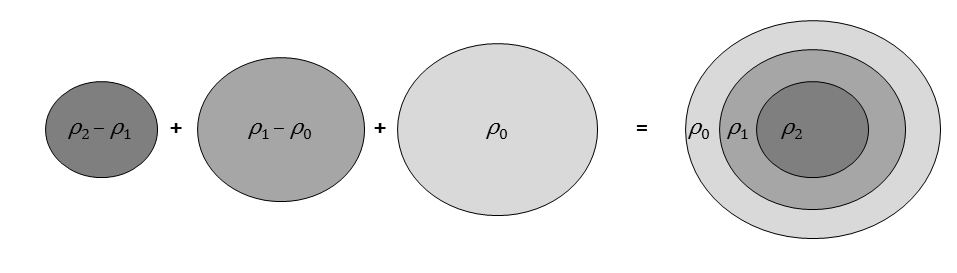
\includegraphics[{width=0.9\textwidth}]{cms_sketch.png}
\caption{Superposition of constant-density spheroids has the same gravitational
potential as a layered spheroid.}
\label{fig:cms_sketch}
\end{figure}

\subsubsection{Definitions}
The spheroids are labeled $i=0,\ldots,N-1$ with the largest, corresponding to the
outermost layer in the layered planet, labeled $i=0$. The equatorial radii are
labeled $a_i$, such that $a_0>a_1>\cdots>a_{N-1}$.
We define $\delta\rho_i=\rho_i-\rho_{i-1}$ for $i>0$ and $\delta\rho_0=\rho_0$.
The surface of spheroid $i$ is given by the function $r_i(\mu=\cos\theta)$ and we
still assume a fluid planet at equilibrium with the associated symmetry. We will
often use dimensionless shape functions $\xi_i=r_i/a_0$.

\subsubsection{The starting point}
The starting point is equations (\ref{eq:simp_sphe_gravity}) reproduced here for
convenience:
\begin{subequations}
\begin{equation}
V(r,\mu)=\frac{G}{r}\sum_{k=0}^{\infty}\left(r^{-2k}D_{2k} +
r^{2k + 1}D'_{2k}\right)P_{2k}(\mu)
\end{equation}
with
\begin{align}
D_k &= \int_{r'<r}\rho(\arp)(r')^kP_k(\mu')\,d\tau',\\
D'_k &= \int_{r'>r}\rho(\arp)(r')^{-k-1}P_k(\mu')\,d\tau'.
\end{align}
\end{subequations}

\subsubsection{The measurable $J_n$ coefficients are the sum of $J_{i,n}$}
By the principal of superposition the total gravitational potential at a point
$(r,\mu)$ away from the planet (so $r'<r$) is
\begin{equation}
V\sub{ext} = \frac{G}{r}\left(\sum_{k=0}^{\inf}D_{0,2k}r^{-2k}P_{2k}(\mu) + 
\sum_{k=0}^{\inf}D_{1,2k}r^{-2k}\ptk(\mu) + \cdots + 
\sumonk{}D_{N-1,2k}r^{-2k}\ptk(\mu) \right)
\end{equation}
with
\begin{equation}
D_{i,2k} = \frac{2\pi\dro_i}{2k + 3}
\int_{-1}^{1}d\mu'\,\ptk(\mu')r_i(\mu')^{2k + 3}
\end{equation}
(see eq.\eqref{eq:polar_integral}). Notice also that
\begin{equation}\label{eq:M_is_sum_on_D0}
\sum_{i=0}^{N-1}D_{i,0} = \sumoni\frac{2\pi\dro_i}{3}\intonmu{d}\mu'\,r_i(\mu')^3
= M.
\end{equation}

The dimensionless coefficients are all normalized by the same radius
\begin{equation}
Ma_0^{2k}J_{i,2k} = -D_{i,2k}
\end{equation}
so that the external potential can be written as
\begin{equation}
V\sub{ext}(r,\mu) = \frac{GM}{r}\left(1 -
\sumoni\sum_{k=1}^{\inf}J_{i,2k}(r/a_0)^{-2k}\ptk(\mu)\right).
\end{equation}
Since the infinite series on $k$ converges\WarningsOff\footnote{Away from the
planet the convergence of the Legendre expansion in $r'/r$ is not in question, so
there is no problem with the claim that the measured $J_n$ are the sum of layer
$J_{i,n}$. But for the actual calculation of $J_{i,n}$ by eq.~\eqref{eq:J_i_2k}
we need the stronger claim that the Legendre expansion in $D$ is valid also on the
surface of the spheroid.}\WarningsOn we can change the order of summation and
write
\begin{equation}
V\sub{ext}(r,\mu) = \frac{GM}{r}\left(1 -
\sum_{k=1}^{\inf}\left(\sumoni{}J_{i,2k}\right)(r/a_0)^{-2k}\ptk(\mu)\right),
\end{equation}
which shows that the coefficients $J_n$ measurable by spacecraft are the simple
algebraic sum of the individual $J_{i,2k}$, given by
\begin{equation}\label{eq:J_i_2k}
J_{i,2k} = -\left(\frac{3}{2k + 3}\right)
\frac{\dro_i\intonmu{d}\mu'\,\ptk(\mu')\xi_i(\mu')^{2k + 3}}
{\sum_{j=0}^{N-1}\dro_j\intonmu{d}\mu'\,\xi_j(\mu')^3}.
\end{equation}
This is the equivalent to eq.~\eqref{eq:Jn_maclaurin_ext} for a single Maclaurin
spheroid.

As before, we will use an iterative process. We will numerically evaluate the
integrals in eq.\eqref{eq:J_i_2k}. The shape functions of the surfaces of the
spheroids, $\xi_i(\mu')$ in the integrands, will be numerically solved using
current values of $J_{i,2k}$, and the process will continue until the coefficients
$J_{i,2k}$ for all layers remain unchanged through successive iterations. However,
unlike in the case of a single spheroid, the $J_{i,2k}$ are not sufficient to
calculate the shape functions of interior spheroids. We need an expression for the
total potential at an interior point on the boundary between spheroid $i$ and
spheroid $i-1$.

\subsubsection{The potential at an interior point}
Consider a point $B=(r_j(\mu),\mu)$ on the level surface of spheroid $j$. The
contribution to the potential from any spheroid $i\ge{j}$ is the external
potential:
\begin{equation}\label{eq:vigtj}
V_{i\ge{j}}(r_j(\mu),\mu) = \frac{G}{r_j}\sumonk{D_{i,2k}}r_j(\mu)^{-2k}\ptk(\mu).
\end{equation}
The contribution from a spheroid $i<j$ has two parts. The external part, from the
sphere of radius $r_j$ inside spheroid $i$:
\begin{equation}
V_{i<j,\mathrm{ext}}(r_j,\mu) = \frac{G}{r_j}\frac{4\pi}{3}\dro_i r_j(\mu)^3.
\end{equation}
And the internal part, from the oblate region in spheroid $i$ where $r'>r_j$:
\begin{equation}
V_{i<j,\mathrm{int}}(r_j,\mu) =
\frac{G}{r_j(\mu)}\sumonk{}r_j(\mu)^{2k+1}\ptk(\mu)\;
2\pi\,\dro_i\intonmu{d}\mu'\,\ptk(\mu')\int_{r_j(\mu)}^{r_i(\mu')}dr'\,
(r')^{-2k-1}(r')^2.
\end{equation}
(Note typo in eq.~(15) of \citep{Hubbard2013}.)

The rest is just algebra but here are a few points to keep in mind while we work.
First, since we now have $r'$ to a negative power in the inner integrand we have
to do the $k=1$ term, the integral of $(r')^{-1}$, separately. Second, the lower
bound of the inner integral is independent or $\mu'$. This means that the outer
integral will have a term that is simply a constant times $\ptk(\mu')$. Recall
that the orthogonality of Legendre polynomials requires that
$\int_{-1}^{1}P_{n>0}(x)\,dx=0$ so that this term is identically zero except when
$k=0$. So we will also need to do the $k=0$ term separately. Third, we will lump
an $r_j^2$ term together with the contribution from $V_{i<j,\mathrm{ext}}$. Also
we will use the oblate symmetry to take the integrals over $\mu$ from $0$ to $1$.
Here we go.

\begin{multline}
V_{i<j,\mathrm{int}}(r_j,\mu) =
\tpi{G}\dro_i\mupint[r_i(\mu')^2 - r_j(\mu)^2]\; +\\
4\pi{G}\dro_i\,r_j(\mu)^2{}P_2(\mu)\mupint{}P_2(\mu')[\ln{r_i(\mu')} -
\ln{r_j(\mu)}\; + \\
\tpi{G}\dro_i\,\sum_{k=2}^{\inf}r_j(\mu)^{2k}\ptk(\mu)\,\frac{2}{2 -2k}
\mupint\ptk(\mu')[r_i(\mu')^{2 - 2k} - r_j(\mu)^{2 - 2k}]\; = \\
\tpi{G}\dro_i\mupint{}r_i(\mu')^2 - \tpi{G}\dro_i{}r_j(\mu)^2\; + \\ 
4\pi{G}\dro_i\,r_j(\mu)^2{}P_2(\mu)\mupint{}P_2(\mu')\ln{r_i(\mu')}\; + \\
2\pi{G}\dro_i\,\sum_{k=2}^{\inf}r_j(\mu)\ptk(\mu)\,\frac{2}{2 - 2k}
\mupint\ptk(\mu')r_i(\mu')^{2 - 2k}.
\end{multline}
And combined with the contribution $V_{i<j,\mathrm{ext}}$ we have
\begin{multline}
V_{i<j} = -\frac{2\pi{G}\dro_i}{3}r_j(\mu)^2 +
2\pi{G}\dro_i\mupint{}r_i(\mu')^2\; + \\
4\pi{G}\dro_i\,r_j(\mu)^2P_2{\mu}\,\mupint{}P_2(\mu')\ln{r_i(\mu')}\; + \\
2\pi{G}\dro_i\,\sum_{k=2}^{\inf}r_j(\mu)^{2k}\ptk(\mu)\,
\frac{2}{2 - 2k}\mupint\ptk(\mu')r_i(\mu')^{2 - 2k}.
\end{multline}

We can write the potential as a sum of powers of $r_j$ with $D$-like coefficients
so that it looks more like eq.~\eqref{eq:vigtj}:
\begin{equation}\label{eq:viltj}
V_{i<j}(r_j(\mu),\mu) = G\sum_{k=0}^{\inf}D'_{i,2k}r_j(\mu)^{2k}\ptk(\mu) + 
G\,D''_{i,0}\,r_j(\mu)^2,
\end{equation}
with
\begin{subequations}
\begin{align}
D'_{i,2k} &= \frac{4\pi}{2 - 2k}\dro_i
\mupint\ptk(\mu')r_i(\mu')^{2 - 2k}, & k\ne{1},\\
D'_{i,2} &= 4\pi\dro_i\mupint{}P_2(\mu')\ln{r_i(\mu')}, & k=1,\\
\intertext{and}
D''_{i,0} &= -\frac{2\pi}{3}\dro_i.
\end{align}
\end{subequations}

For the non-dimensional coefficients let
\begin{subequations}
\begin{align}
Ma_0^{2k}J_{i,2k} &= -D_{i,2k},\\
Ma_0^{-(2k+1)}J'_{i,2k} &= -D'_{i,2k},\\
\intertext{and}
Ma_0^{-3}J''_{i,0} &= -D''_{i,0},
\end{align}
\end{subequations}
and eqs.~\eqref{eq:vigtj} and~\eqref{eq:viltj} become
\begin{equation}
V_{i\ge{j}} = -\frac{GM}{r_j}
\sumonk{}J_{i,2k}\Bigl(\frac{r_j}{a_0}\Bigr)^
{-2k}\ptk(\mu)
\end{equation}
and
\begin{equation}
V_{i<j} = -\frac{GM}{r_j}\left[
\sumonk{}J'_{i,2k}\Bigl(\frac{r_j}{a_0}\Bigr)^{2k+1}\ptk(\mu) +
J''_{i,0}\Bigl(\frac{r_j}{a_0}\Bigr)^3 \right].
\end{equation}

And finally, we put it all together. Using non-dimensional coefficients and the
normalized radius $\xi=r/a_0$, the total gravitational potential at point
$B=(\xi_j(\mu),\mu)$ on the equilibrium surface of spheroid $j$ summing
contributions from all spheroids is
\begin{equation}\label{eq:VatB}
\begin{split}
V(\xi_j,\mu) = 
-\frac{GM}{a_0}\frac{1}{\xi_j(\mu)}\Biggl[
&\sum_{i=j}^{N-1}\sumonk{}J_{i,2k}\xi_j(\mu)^{-2k}\ptk(\mu)\; + \\
& \sum_{i=0}^{j-1}\sumonk{}J'_{i,2k}\xi_j(\mu)^{2k+1}\ptk(\mu) + 
  \sum_{i=0}^{j-1} J''_{i,0}\xi_j(\mu)^3
\Biggr].
\end{split}
\end{equation}
With the coefficients
\begin{subequations}\label{eq:J_menagerie}
\begin{align}
J_{i,2k} &= -\left(\frac{3}{2k + 3}\right)
\frac{\dro_i\mupint\ptk(\mu')\xi_i(\mu')^{2k + 3}}
{\sum_{m=0}^{N-1}\dro_m\mupint\xi_m(\mu')^3},\\
J'_{i,2k} &= -\left(\frac{3}{2 - 2k}\right)
\frac{\dro_i\mupint\ptk(\mu')\xi_i(\mu')^{2 - 2k}}
{\sum_{m=0}^{N-1}\dro_m\mupint\xi_m(\mu')^3}, & k\ne{1},\\
J'_{i,2} &= -3\;
\frac{\dro_i\mupint{}P_2(\mu')\ln{\xi_i(\mu')}}
{\sum_{m=0}^{N-1}\dro_m\mupint\xi_m(\mu')^3}, & k=1,\\
J''_{i,0} &= \frac{1}{2}\;
\frac{\dro_i}{\sum_{m=0}^{N-1}\dro_m\mupint\xi_m(\mu')^3}.
\end{align}
\end{subequations}
(For the surface, $j=0$ layer the second double sum in~\eqref{eq:VatB} is
dropped.)

\subsubsection{A self-consistent interior model}

With eq.~\eqref{eq:VatB} at hand we can construct a self-consistent shape for an
array of $N$ layers with densities $\rho_i$ and equatorial radii $a_i$, given a
rotation parameter $q$. We use an iterative method similar to the one in
sec.~\ref{sec:a_constant_density_spheroid}. Start with an initial guess for the
values of all $J$-like coefficients in eqs.~\eqref{eq:J_menagerie}. The simplest
guess is to use values corresponding to a perfectly spherical planet:
$J_{i,0}=-(\rho_i-\rho_{i-1})/\rho_{N-1}$, $J'_{i,0}=(3/2)J_{i,0}$,
$J''_{i,0}=-(1/2)J_{i,0}$, and all other coefficients equal to zero. We then
reevaluate all the coefficients by numerically integrating
eqs.~\eqref{eq:J_menagerie}. To evaluate the integrands we need the shape
functions, $\xi_i(\mu')$. We obtain those using the \emph{current} values of the
$J$-coefficients. The implicit equations defining the shape functions are obtained
by equating the \emph{total} potential (including a centrifugal term) at
$(\xi_i(\mu'),\mu')$ to the value computed at $(a_i/a_0,0)$. An implicit equation
is solved, numerically, for every point where an integrand is evaluated in each of
eqs.~\eqref{eq:J_menagerie} so this will be a computationally expensive operation.
The result of an iteration is a new set of values for $J$ coefficients. The next
iteration will use these new values when computing the shape functions, and will
therefore return slightly different updated values for $J$s. Iterations continue
until successive updates no longer modify any $J$ above the specified tolerance.

The resulting converged model is a self-consistent mass distribution. In other
words, the shape of the layered spheroid is such that gravitational accelerations
balance centrifugal accelerations everywhere. However the mass distribution is
probably not consistent with a realistic equation-of-state. Indeed up to now the
composition of the planet was not even mentioned. To obtain a useful interior
model of a fluid planet we employ a second level of iterations. Computing the
pressure inside layers of constant density (by integrating, numerically, from the
surface down) we compare the value to the pressure predicted by a chosen barotrope
meant to represent the planet's composition, and adjust the layer densities
accordingly. We then run the first level iterations again to converge again to a
self-consistent mass distribution, and repeat the process until successive
iterations no longer modify the layer densities above a specified tolerance.

In principle this completes the description of the concentric Maclaurin spheroid
technique for modeling a rotating fluid. However there are many details that are
useful to consider when implementing the method in practice, and some that are
necessary. These are the subject of part~\ref{part:practice}.

% subsection concentric_maclaurin_spheroids (end)

\section{Practice\label{part:practice}}
As always, when we begin to implement a theoretical model as an actual computer
program we discover many small details that are not particularly important or
interesting for a general understanding of the theory but are nonetheless
necessary to consider for a practical implementation. I describe those here using
the notation of \citet{Hubbard2013} which I am hoping will become standard
notation for CMS models. I also mention some details that are particular to my
MATLAB implementation, \ML{set apart like this.}

\subsubsection{Truncating infinite series}

\red{Look at eq.~\eqref{eq:VatB}. Obviously we must truncate the series at some
$k=\kmax$. But how to choose $\kmax$ for the desired accuracy? It's easier to
experiment than it is to analyze, and it turns out that truncating at
$n=2\kmax=30$ leaves a remainder of $\about{10^{-12}}$.}

\subsubsection{Rescaling}

Suppose we want to construct a modest CMS model with $N=100$ layers and
$\kmax=15$. Look at eq.~\eqref{eq:VatB}, for the $j=100$ layer. The $k=10$ term in
the first double sum contains a product of $J_{100,20}$ and the huge number
$\xi_{100}(\mu)^{-20}\sim(10^{-2})^{-20}$. But look now at
eqs.~\eqref{eq:J_menagerie}. The integrand in the expression for $J_{100,20}$ is
on the order $\about(10^{-2})^{23}$, more than enough to subdue the huge value of
$\xi^{-2k}$ and make the contribution to the potential from the degree 20 moment
of the smallest layer negligible, as expected. Similarly, when we come to
calculate, say, $J'_{100,20}$ the integrand is huge, of order
$\about{}(10^{-2})^{-18}$, and the corresponding term in eq.~\eqref{eq:VatB}
is a product of this huge number with a factor of order $\about{}(10^{-2})^{21}$,
so that the contribution to the potential is again small, as expected. This is
fine in principle, but in practice in order to preserve numerical accuracy it is
important to avoid multiplying and dividing by huge numbers. We can do this by
rescaling the dimensionless multipole moments and associated equations.

Define $\lambda_i\equiv(a_i/a_0)$ and $\zeta_i\equiv\xi_i/\lambda_i=r_i/a_i$. I
call $\zeta_i(\mu)$ the \emph{renormalized shape functions}. Notice that $\zeta_i
(\mu')\lesssim{1}$, always. In the definition of the $J'_{100,20}$, for example,
the large numerical value can be pulled out of the integral:
\begin{equation*}
J'_{i,2k} = -\left(\frac{3}{2 - 2k}\right)
\frac{\dro_i\lambda_i^{2 - 2k}\mupint\ptk(\mu')\zeta_i(\mu')^{2 - 2k}}
{\sum_{m=0}^{N-1}\dro_m\lambda_m^3\mupint\zeta_m(\mu')^3}, \qquad k\ne{1},
\end{equation*}
the expected huge value now coming from $\lambda_i^{2-2k}$. We can prevent
multiplication by this huge value by rescaling the mulipole moment itself.
Defining $\Jtil'_{i,2k}=J'_{i,2k}\lambda_i^{2k+1}$, the potentially huge number is
deferred, we shall see, to the expression for the potential where, we shall see,
it is subdued by an even larger number, avoiding the expected loss of accuracy.
Similarly, the $J_{i,2k}$ moments are rescaled to
$\Jtil_{i,2k}=J_{i,2k}/\lambda^{2k}$ to match the change of variables from $\xi$
to $\zeta$. And although the rescaling is not necessary for numerical reason in
the case of $J''_{i,0}$ we do not want to maintain two sets of variables so we
perform the same change of variables and rescaling moments by
$\Jtil''_{i,0}=J''_{i,0}\lambda_i^3$. Eqs.~\eqref{eq:J_menagerie} are then
replaced by eqs.~\eqref{eq:rescaledJs}, involving no numerically huge numbers:
\begin{subequations}\label{eq:rescaledJs}
\begin{align}
\Jtil_{i,2k} &= -\left(\frac{3}{2k + 3}\right)
\frac{\dro_i\lambda_i^3\mupint\ptk(\mu')\zeta_i(\mu')^{2k + 3}}
{\sum_{m=0}^{N-1}\dro_m\lambda_m^3\mupint\zeta_m(\mu')^3},\\
\Jtil'_{i,2k} &= -\left(\frac{3}{2 - 2k}\right)
\frac{\dro_i\lambda_i^3\mupint\ptk(\mu')\zeta_i(\mu')^{2 - 2k}}
{\sum_{m=0}^{N-1}\dro_m\lambda_m^3\mupint\zeta_m(\mu')^3}, & k\ne{1},\\
\Jtil'_{i,2} &= -3\;
\frac{\dro_i\lambda_i^3\mupint{}P_2(\mu')\ln{\zeta_i(\mu')}}
{\sum_{m=0}^{N-1}\dro_m\lambda_m^3\mupint\zeta_m(\mu')^3}, & k=1,\\
\Jtil''_{i,0} &= \frac{1}{2}\;
\frac{\dro_i\lambda_i^3}{\sum_{m=0}^{N-1}\dro_m\lambda_m^3\mupint\zeta_m(\mu')^3}.
\end{align}
\end{subequations}
(To understand the $k=1$ term recall that $\int_0^1P_2(\mu')\,d\mu'=0$.)

Now, in terms of the renormalized shape functions and the rescaled multipole
moments eq.~\eqref{eq:VatB} is replaced by:
\begin{equation}\label{eq:VpuatB}
\begin{split}
V\sub{pu}(\zeta_j,\mu) = \frac{a_0}{GM} V(\zeta_j,\mu) &= \\ 
-\frac{1}{\lambda_j\zeta_j(\mu)}\Biggl[
&\sum_{i=j}^{N-1}\sumkmax{}\Bigl(\frac{\lambda_i}{\lambda_j}\Bigr)^{2k}
\Jtil_{i,2k}\zeta_j(\mu)^{-2k}\ptk(\mu)\; + \\
&\sum_{i=0}^{j-1}\sumkmax{}\Bigl(\frac{\lambda_j}{\lambda_i}\Bigr)^{2k+1}
\Jtil'_{i,2k}\zeta_j(\mu)^{2k+1}\ptk(\mu) + 
\sum_{i=0}^{j-1}\Bigl(\frac{\lambda_j}{\lambda_i}\Bigr)^3
\Jtil''_{i,0}\zeta_j(\mu)^3
\Biggr].
\end{split}
\end{equation}
Notice how the ratios of $\lambda$s in the double sums are always less than or
equal to one, and the $\zeta$ shape functions also have values close to but less
than one, as long as the oblateness is not extreme. In this form it is easy to see
that the expansions in multipole moments, with expressions \eqref{eq:rescaledJs}
for the coefficients, are expected to converge rapidly, allowing us to choose a a
sensible $\kmax$. We also introduced the non-dimensional potential $V\sub{pu}$.
The subscript stands for planetary units.

% References
\bibliographystyle{plainnat} % [plainnat|abbrvnat|agu08|agufull08|...]
\bibliography{/users/naor/documents/library}

% ----------------------------------------------------------------
\end{document}
% ----------------------------------------------------------------
%END OF FILE
%-----------------------------------------------------------------
